% \section{Introduction}
%
% - \texit{Ab initio} structure prediction is a balancing act between time spent to generate decoys and the quality of the final decoy set
% - \texit{Ab initio} structure prediction can only predict accurate structures with a subselection of fragments collective capturing the overall target fold
%
% - AMPLE requires decoys with the overall accurate fold yet enough diversity in the set to truncate to the conserved core
% - AMPLE typically succeeds with small to medium size fragments relative to the target sequence (20-50\%)
%
% This bares the question whether fragments extracted for \texit{ab initio} structure prediction are sufficient as MR search models. This stems primarily on the assumption that fragment picking algorithms can identify fragments based on sequence features that are structurally similar to a sequence position in our target.
%
% - Something about the addition of contacts as unique feature for further identifying correct fragments
% - Something about differences to other fragment-MR approaches

\section{Methods}
\subsection{Target selection}
Targets were manually chosen using favourable cases for this proof-of-principle study, i.e. resolution was chosen to be ~1.5\AA, target chain lengths were $<150$ residues, and only a single molecule is present in the asymmetric unit (Table \ref{table:ample_flib_target_properties}).

\begin{table}[H]
  \centering
  \begin{tabularx}{\textwidth}{|X|X|X|X|X|X|}
      \hline
      \textbf{Target} & \textbf{Fold} & \textbf{Chain Length} & \textbf{Resolution (\AA)} & \textbf{Nmol/ASU} &
\textbf{Space Group} \\ 
      \hline
      1aba & mixed \textalpha-\textbeta & 87    & 1.45 & 1      & P $2_1$ $2_1$ $2_1$   \\ \hline
      1lo7 & mixed \textalpha-\textbeta & 141   & 1.50 & 1      & I $2$ $2$ $2$         \\ \hline
      1u06 & all-\textbeta              & 62    & 1.49 & 1      & P $2_1$ $2_1$ $2_1$   \\ \hline
      5nfc & all-\textbeta              & 147   & 1.59 & 1      & P $2_1$ $2_1$ $2_1$   \\ \hline
  \end{tabularx}
  \caption{Overview of Flib target properties.}
  \label{table:ample_flib_target_properties}
\end{table}

\subsection{Fragment picking using Flib}
Fragments for this study were picked using the Flib algorithm \cite{De_Oliveira2015-ba}. 

Flib requires four inputs: the predicted secondary structure, predicted torsion angles, predicted residue-residue contact prediction and a copy of the \gls{pdb}. The secondary structure for each target was predicted using PSIPRED v4.0 \cite{Jones1999-fi} with default parameters. The torsion angles were predicted using SPIDER2 \cite{Heffernan2015-wp} with default parameters, and residue-residue contact pairs using METAPSICOV v1.04 \cite{Jones2015-wp} with default parameters. HHBLITS v2.0.16 \cite{Remmert2011-ze} with database version \texttt{uniprot20\_2016\_02} was used by METAPSICOV to generate the \gls{msa} for contact prediction of each target sequence. BLASTp v2.2.31+ was used by PSIPRED with the UNIPROT database version \texttt{uniref90-2016\_06}. The local copy of the \gls{pdb} for fragment picking was downloaded on August 11, 2016.

Two modifications were made to the default Flib v1.01 (\url{https://github.com/sauloho/Flib-Coevo}) protocol. The first focuses on exclusion of fragments with $>90$\% helical content (assigned by DSSP \cite{Frishman1995-ns}). The second modification was to allow fragments with \gls{rmsd} $>10.0$\AA\ to be considered.

Two-hundred fragments were picked per target sequence position. Top-$L$ or $L/2$ contact pairs were considered from both METAPSICOV STAGE 1 and STAGE 2 predictions with a minimum sequence separation of either 6 or 12 residues. Helical fragments were either in- or excluded and only fragments with length between 6 or 12 residues up-to 63 residues considered. Overall, this generated 16 fragment libraries per target.

Each fragment library was then filtered to remove homologs. Hereby, BLASTp \cite{Altschul1990-nc} and HHpred \cite{Soding2005-sx} searches were conducted to identify homologous PDB entries. The BLASTp search was performed identically to \cite{De_Oliveira2015-ba}. The HHpred search parameters were identical to the MPI-Toolkit \cite{Biegert2006-ny} webserver version (\url{https://toolkit.tuebingen.mpg.de/}). Fragments derived from PDB entries identified by BLASTp and HHpred (probability score of $\geq20.0$) were excluded from the fragment libraries.

All fragments per target were then grouped by their length. Subsequently, they were ranked twice by Flib scores and \gls{rmsd} values, and the best fragment selected. The coordinates for the selected fragments were then extracted and two versions for each file created, once containing backbone atoms only and once containing all atoms.

\subsection{Molecular Replacement in MrBUMP}
The previously extracted fragments were subjected to the MR pipeline MrBUMP \cite{Keegan2008-hk}. The latter uses PHASER \cite{McCoy2007-bf} for MR, REFMAC5 \cite{Murshudov2011-we} for refinement and SHELXE \cite{Thorn2013-ir} for density modification and main-chain tracing. MrBUMP default parameters were used with exception of the PHASER RMS estimate. MR was attempted for each coordinate file with a PHASER RMS value of 0.1, 0.6, and 1.0.

The MR success for each search model was assessed by SHELXE scores only. Hereby, a SHELXE \gls{cc} score of $\geq25.0$ was required combined with an \gls{acl} score of $\geq10.0$.


\section{Results}
\subsection{Precision of Flib dependency data}
The first part of this study is to analyse the data dependencies required by the Flib fragment picking algorithm. This analysis is important given that the Flib fragment picking heavily relies on the individual features in the selection and scoring of each individual fragment \cite{De_Oliveira2015-ba}. Poor data at this stage could lead to poor fragments unsuitable for MR trials, given that high accuracy, i.e. a low \gls{rmsd} between the search model and target are required \cite{} (<-- Phaser paper here).

The secondary structure prediction highlighted high precision between each target's prediction and the DSSP-assigned \cite{Frishman1995-ns} secondary structure of the target reference structure (Fig \ref{fig:ample_flib_psipred}). The three targets with \gls{pdb} identifiers 1aba, 1lo7 and 1u06 have secondary structure predictions with a precision of $>72$\%. The fourth target, 5nfc, shows comparatively poor precision of 52.4\%. However, almost all secondary structure features are correctly identified. Furthermore, a total of nine residues are missing from the target \gls{pdb} structure, thus lowering the precision score by 5\% (<-- double-check).

\begin{figure}[H]
	\centering
	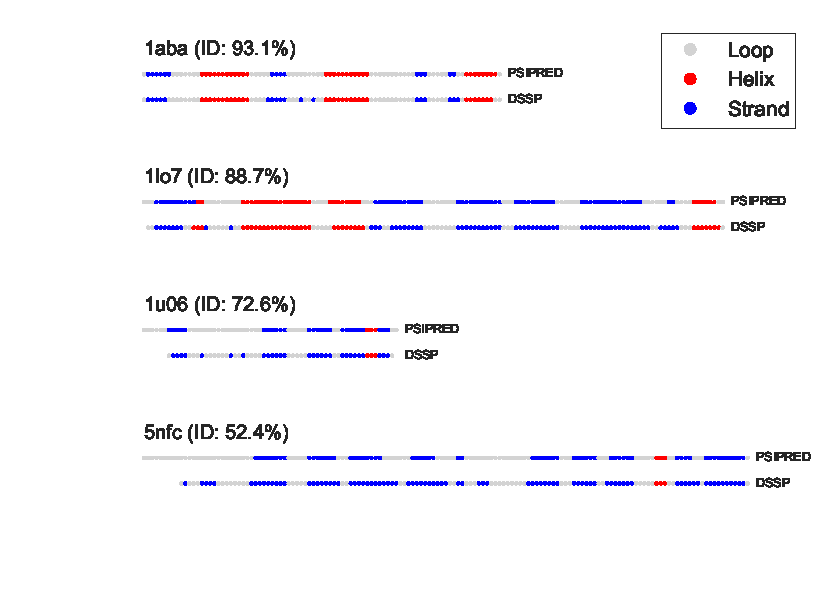
\includegraphics[width=\textwidth]{ample_flib_psipred.pdf}
	\caption{Schematic comparison of PSIPRED \cite{Jones1999-fi} secondary structure prediction and DSSP \cite{Frishman1995-ns} assignment. Percentage identity is provided next to each identifier.}
	\label{fig:ample_flib_psipred}
\end{figure}

The contact prediction data for METAPSICOV STAGE 1 and STAGE 2 predictions demonstrate the high precision scores achievable by this algorithm (Table \ref{table:ample_flib_contact_precision}). In this study, the top contact pairs at cutoffs \textit{L} and \textit{L/2} were provided to the Flib algorithm. All targets have precision scores for both sets of predictions at both cutoff levels of $>0.6$ (Table \ref{table:ample_flib_contact_precision}).

% This needs to be fixed. Put across the top the number of contacts selected and reduce the width of the empty column. Maybe some summary statistics?
\begin{table}[H]
  \centering
  \begin{tabularx}{\textwidth}{|X|X|X|X|X|X|X|}
      \hline
	  \multirow{2}{*}{\textbf{Target}} & \multicolumn{3}{c|}{\textbf{\textit{L/2} contact pairs}} & \multicolumn{3}{c|}{\textbf{\textit{L} contact pairs}} 				\\ \cline{2-7}
	  							&  	STAGE 1	& 	STAGE 2	& 	Jaccard 	& 	STAGE 1 	& 	STAGE 2 	& 	Jaccard	 	\\ \hline
	  1aba						&	0.884	&	0.884	&	0.303	&	0.713	&	0.759	&	0.513		\\ \hline
	  1lo7						&	0.857	&	0.957	&	0.308	&	0.738	&	0.837	&	0.446		\\ \hline
	  1u06						&	0.839	&	0.806	&	0.378	&	0.710	&	0.787	&	0.459		\\ \hline
	  5nfc						&	0.822	&	0.836	&	0.327	&	0.619	&	0.762	&	0.434		\\ \hline
  \end{tabularx}
  \caption[Contact prediction summary for Flib targets]{Precision scores for METAPSICOV \cite{Jones2015-wp} STAGE 1 and STAGE 2 contact predictions. Jaccard index calculated for the same contact pairs between METAPSICOV STAGE 1 and STAGE 2 predictions.}
  \label{table:ample_flib_contact_precision}
\end{table}

The torsion angle analysis ...

% \subsection{Flib fragment picking}
% - Overall distribution of Flib and \gls{rmsd} scores (also by target)
% - Which parameter combination picks fragments with lowest Flib scores




